\documentclass[]{article}
\usepackage{amsmath,amsfonts,pstricks,pst-eps,tikz,verbatim,mathtools}
\pagestyle{empty}
\title{Final project}
\author{Jiawen Bi}
\date{\today}
\begin{document}
\maketitle
The whole function is $$
    P(x) = \sum_{i=0}^n P_i F_i^k(x)
   	$$
where $P_i$ is the de Boor point, $F_i^k(x)$ is the basis function according to the handout. 
I am going to use the cubic B-spline curve to fit the pattern.
We know according to Example 4.26 that the basis quadratic B-spline $$
	B_i^2(x) = \begin{dcases}
	\frac{(x-t_{i-1})^2}{(t_{i+1}-t_{i-1})(t_i - t_{i-1})} & x\in \left(t_{i-1},t_i\right] \\
	\frac{(x-t_{i-1})(t_{i+1}-x)}{(t_{i+1}-t_{i-1})(t_{i+1}-t_i)} + \frac{(t_{i+2}-x)(x-t_i)}{(t_{i+2}-t_i)(t_{i+1}-t_i)} & x\in \left(t_i,t_{i+1}\right] \\
	\frac{(t_{i+2}-x)^2}{(t_{i+2}-t_i)(t_{i+2}-t_{i+1})} & x\in \left(t_{i+1},t_{i+2} \right] \\
	0 & otherwise
	\end{dcases}
$$
and according to Definition 4.24, $$
	B_i^{n+1}(x) = \frac{x-t_{i-1}}{t_{i+n}-t_{i-1}}B_i^n(x) + \frac{t_{i+n+1} - x}{t_{i+n+1}-t_i} B_{i+1}^n(x)
$$
so we can get the basis cubic B-spline $$
	B_i^3(x) = \begin{dcases}
	\frac{(x-t_{i-1})^3}{(t_{i+2}-t_{i-1})(t_{i+1}-t_{i-1})(t_i-t_{i-1})} & \left(t_{i-1},t_i\right] \\
	\frac{(t_{i+1}-x)(x-t_{i-1})^2}{(t_{i+1}-t_i)(t_i-t_{i-1})(t_{i+1}-t_{i-1})} + \frac{(x-t_{i-1})^2(t_{i+1}-x)}{(t_{i+2}-t_{i-1})(t_{i+1}-t_{i-1})(t_{i+1}-t_i)} & \cdots \\ 
	 + \frac{(t_{i+2}-x)(x-t_i)(x-t_{i-1})}{(t_{i+2}-t_i)(t_{i+1}-t_i)(t_{i+2}-t_{i-1})} & \left(t_i,t_{i+1} \right] \\
	\frac{(t_{i+2}-x)^2(x-t_{i-1})}{(t_{i+2}-t_{i-1})(t_{i+2}-t_i)(t_{i+2}-t_{i+1})} + \frac{(t_{i+3}-x)(x-t_{i-1})(t_{i+1}-x)}{(t_{i+1}-t_{i-1})(t_{i+1}-t_i)(t_{i+3}-t_i)} & \cdots\\
	+\frac{(t_{i+3}-x)(t_{i+2}-x)(x-t_i)}{(t_{i+3}-t_i)(t_{i+2}-t_i)(t_{i+1}-t_i)} & \left(t_{i+1},t_{i+2} \right] \\
	\frac{(t_{i+3}-x)(t_{i+2}-x)^2}{(t_{i+3}-t_i)(t_{i+2}-t_i)(t_{i+2}-t_{i+1})} & \left(t_{i+2},t_{i+3} \right]
	\end{dcases}
$$
since $\displaystyle P(x) = \sum P_iB_i^3(x) $, thus for every interval$\displaystyle\left(t_{i-1},t_i\right]$,
\begin{align*}
	P(x) &= P_iB_i^3(x) + P_{i-1}B_{i-1}^3 + P_{i-2}B_{i-2}^3 + P_{i-3}B_{i-3}^3 \\
	&= P_i\frac{x^3 - 3t_{i-1}x^2 + 3t_{i-1}^2x - t_{i-1}^3}  {(t_{i+2} - t_{i-1})(t_{i+1} - t_{i-1})(t_i - t_{i-1})} \\
	&+ P_{i-1}\frac{-x^3 + (2t_{i-2}+t_{i+2})x^2 - (t_{i-2}^2+2t_{i-2}t_{i+2})x + t_{i+2}t_{i-2}^2}  {(t_{i+2} - t_{i-1})(t_{i-1} - t_{i-2})(t_i - t_{i-2})} \\
	&+ P_{i-1}\frac{-x^3 + (2t_{i-2}+t_i)x^2 - (t_{i-2}^2+2t_{i-2}t_i)x + t_{i-2}^2t_i}  {(t_{i+1} - t_{i-2})(t_i - t_{i-2})(t_i-t_{i-1})} \\
	&+ P_{i-1}\frac{-x^3 + (t_{i-1}+t_{i+1}+t_{i-2})x^2 - (t_{i-1}t_{i+1}+t_{i-2}t_{i-1}+t_{i-2}t_{i+1})x-t_{i-1}t_{i+1}t_{i-2}}  {(t_{i+1}-t_{i-1})(t_i-t_{i-1})(t_{i-1}-t_{i-2})} \\
	&+ P_{i-2}\frac{x^3 - (2t_i+t_{i-3})x^2 + (t_i^2+2t_it_{i-3})x - t_i^2t_{i-3}}{(t_i-t_{i-3})(t_i-t_{i-2})(t_i-t_{i-1})} \\
	&+ P_{i-2}\frac{x^3 - (t_{i+1}+t_{i-1}+t_{i-3})x^2 + (t_{i-1}t_{i+1}+t_{i+1}t_{i-3}+t_{i-1}t_{i-3})x - t_{i+1}t_{i-1}t_{i-3}}  {(t_{i-1}-t_{i-3})(t_{i-1}-t_{i-2})(t_i-t_{i-2})} \\
	&+ P_{i-2}\frac{x^3 - (t_i+t_{i+1}+t_{i-2})x^2 + (t_it_{i-1}+t_it_{i-2}+t_{i+1}t_{i-2})x - t_it_{i+1}t_{i-2}}  {(t_{i+1}-t_{i-2})(t_i-t_{i-2})(t_{i-1}-t_{i-2})} \\
	&+ P_{i-3}\frac{-x^3 + (2t_{i-1}+t_i)x^2 - (t_{i-1}^2+2t_it_{i-1})x + t_{i-1}^2t_i}  {(t_i-t_{i-3})(t_{i-1}-t_{i-3})(t_{i-1}-t_{i-2})}
\end{align*}


	
\begin{comment}
\begin{TeXtoEPS}

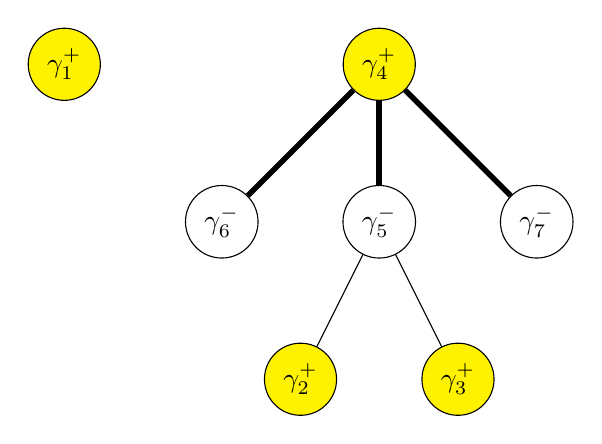
\begin{tikzpicture}
\node[circle,draw,fill=yellow](n4) at (0,0)
	{$\gamma_4^+$};
\node[circle,draw](n6) at (-2,-2) {$\gamma_6^-$}; 
\node[circle,draw](n5) at (0,-2) {$\gamma_5^-$}; 
\node[circle,draw](n7) at (2,-2) {$\gamma_7^-$}; 
\node[circle,draw,fill=yellow](n2) at (-1,-4) {$\gamma_2^+$}; 
\node[circle,draw,fill=yellow](n3) at (+1,-4) {$\gamma_3^+$}; 
\node[circle,draw,fill=yellow](n1) at (-4,0) {$\gamma_1^+$}; 
\draw[line width=2] (n4)--(n6); 
\draw[line width=2] (n4)--(n5); 
\draw[line width=2] (n4)--(n7); 
\draw (n5)--(n2); \draw (n5)--(n3);
\end{tikzpicture}


\end{TeXtoEPS}
\end{comment}
\end{document}

